\documentclass[../main]{subfiles}

\begin{document}

\chapter{The Scratch programming language}\label{ch:scratch-the-programming-language}

\dictum[S. Papert \\ \textit{Mindstorms}]{In teaching the computer how to think, children embark on an exploration about how they themselves think.}

This chapter is a short introduction to Scratch, both the programming language and the environment.
It also explains how the source code for Scratch is organized.

\section{The Scratch environment}\label{sec:scratch-environment}

Scratch is a visual programming language and environment~\autocite{resnickScratchProgrammingAll2009}.
It is block-based, meaning code is represented by blocks with different shapes.
Developed by the Lifelong Kindergarten research group at the MIT Media Lab, beginning in 2002.
Scratch became publicly available in 2007, and has been developed by the Scratch Foundation since 2009.
Its target audience is ages 8 to 16, although it is most commonly used for ages 10 to 14.

\makenote*{The TIOBE index is not that useful: it is based on the number of reported results in search engines~\autocite{bunceTIOBENotTIOBE2008,sundarramPleaseStopCiting2022}. For example, it is known that the Delphi community games or gamed the system~\autocite{bunceTIOBEIndexBeing2009}.}
It is a widely used programming language: the 2022 annual report of the Scratch Foundation~\autocite{GrowingGlobalCreative2022} states that there are over 50 million users in the online Scratch community, with 120 new projects (the programs) being made.
The TIOBE index for March 2024 ranks it as the ninth most used programming language~\autocite{TIOBEIndexMarch2024}.

\begin{figure}
    \begin{wide}
        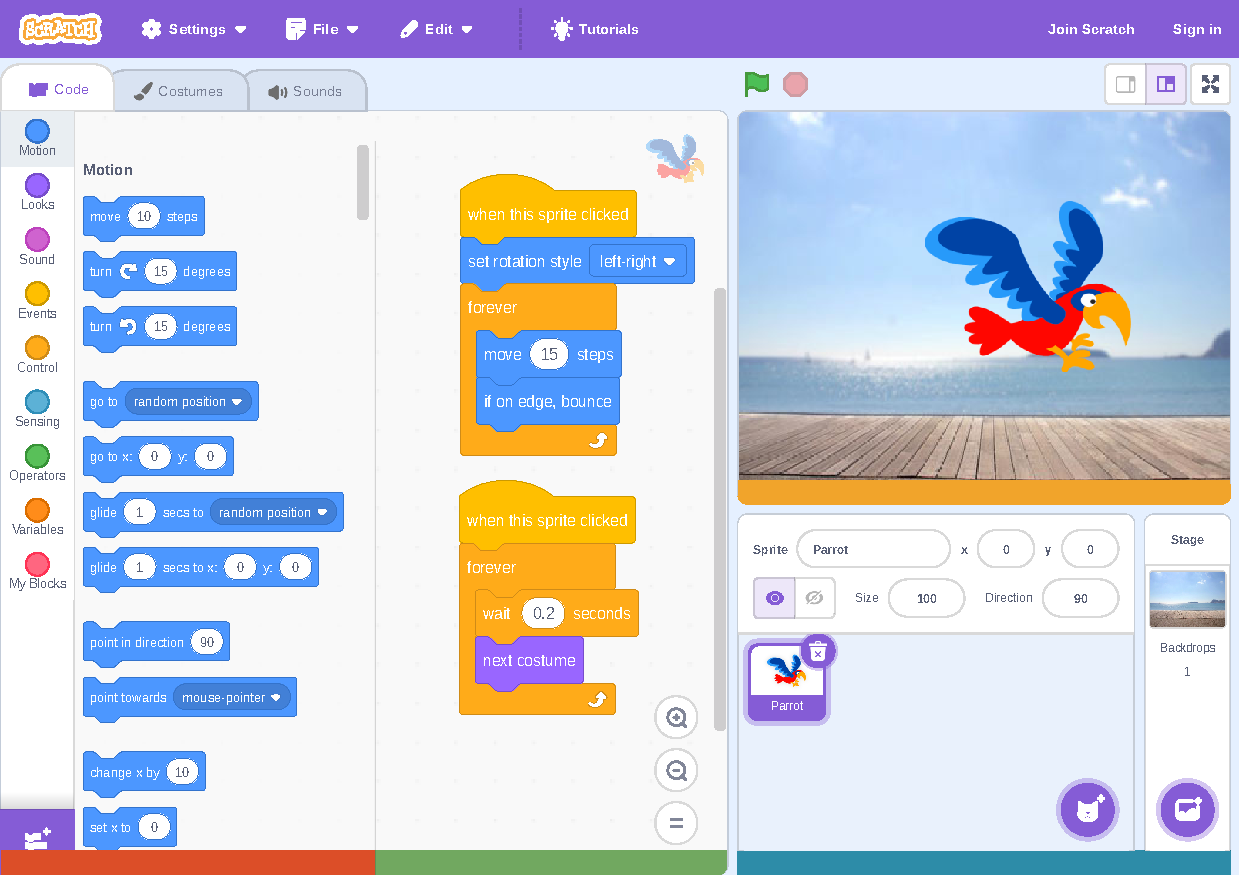
\includegraphics[width=\linewidth]{./scratch-ide}
    \end{wide}
    \caption{The Scratch environment running an example project.
    The toolbox with the available blocks is underlined in \textcolor{ugent-re}{red}, the workspace is underlined in \textcolor{ugent-ps}{green}, the editors for the sprites and the stage are underlined in \textcolor{ugent-we}{blue}, and the canvas is underlined in \textcolor{ugent-lw}{orange}.}
    \label{fig:scratch-environment}
\end{figure}

\subsection{Using the environment and the blocks}\label{subsec:using-the-environment-and-the-blocks}

Blocks can be dragged from the toolbox on the left side of the integrated development environment (\cref{fig:scratch-environment}) to the workspace in the middle and can be stacked together to form scripts.
Blocks can be categorized by their subject or goal: \textcolor{scrmove}{motion}, \textcolor{scrlook}{looks}, \textcolor{scrsound}{sound}, \textcolor{screvent}{events}, \textcolor{scrcontrol}{control}, \textcolor{scrsensing}{sensing}, \textcolor{scroperator}{operators}, \textcolor{scrvariable}{variables}, and \textcolor{scrmoreblocks}{my blocks} (not counting extensions).
Each category has its own colour, except for the blocks that handle lists, as these appear in the \textcolor{scrvariable}{Variables} category, but have a different colour.

Each script starts with a hat block that defines when the script should execute.
Scripts can be started as a result of a user action or when a certain criterium is met during the execution of a program, for example, when a clone is started or a message is broadcast.
A common way to start scripts is to press the green flag (\greenflag), which has two functions: it will first stop all running scripts before starting all relevant hat blocks.
The red stop button next to the green flag also stops all currently running scripts.
The green flag button has another functionality: when there are active scripts, the button gets a darker background colour, even if those scripts were not started by the green flag.

Blocks (or parts of scripts) can also be run independently by clicking them.
This indicates already that Scratch is always live: once a project has been loaded, the virtual machine is always running.
Sprites can be moved or manipulated by the user at any time, even if scripts are running.

Each script is connected to a sprite.
Sprites are objects that are drawn on the screen.
The bottom right corner of the environment contains an editor for sprites and the background, which is a special sprite called Stage that is present in every Scratch project.
All scripts corresponding to the selected sprite are shown in the workspace (middle).
The canvas in the top right corner of the environment shows the execution of the project.

Besides the tab for the blocks (the ``code''), there are also tabs for the costumes and sounds.
The costumes are the visual representation of the sprite.
While some blocks control which costume is used, the list of possible costumes must be prepared in this tab in advance.
The sound tab is very similar, but for sounds instead of costumes.

Finally, users can manage the sprites and stage in the bottom right.
Sprites can be added and removed (even all sprites) by the user.
Similarly, the ``backdrop'' of the stage (which acts as the costume for the stage) can be modified as well.
Note that the stage cannot be removed.

\subsection{Available data types}\label{subsec:scratch-data-types}

Scratch has support for three data types: strings, booleans, and numbers~\autocite{maloneyScratchProgrammingLanguage2010a}.
A different shape is used for booleans (a mix between rectangle and diamond) and strings/numbers (round oval).
Variables and reporter blocks (which are special blocks that result in some value) can only be slotted in boolean slots if the shapes match.
The string/number slots are less strict: if necessary, Scratch will coerce the variable into the right type.

\subsection{Sprites, the object model}\label{subsec:sprites-the-object-model}

Sprites are very similar to objects in Scratch~\autocite{maloneyScratchProgrammingLanguage2010a}.
As all scripts belong to a particular sprite, almost all blocks only work for the current sprite.
Apparently, an earlier version of Scratch had cross-sprite commands, but users found it confusing.

The strict separation of code between sprites means there is a lot of work needed to make a bunch of sprites behave the same way.
For example, a firework might need hundreds of sprites to represent the particles.
Copying all clones by hand quickly becomes tedious.
That is why Scratch has a clone feature: a ``shadow'' sprite is created, whose code is a clone of the original.
This clone is not visible in the sprite overview, only on the canvas.

Variables are normally also limited to the sprite that defined them and are not visible to other sprites.
There is an exception: the variables of the stage are visible to all sprites, and could thus also be used for inter-sprite communications.

\subsection{Inter-sprite communications}\label{subsec:intersprite-communications}

\textcolor{screvent}{Broadcasts} are the intended way to let sprites communicate with each other.
There are other ways, such as global variables or implicit communication (for example, blocks that trigger when a colour is touched).
However, broadcasts remain the intended way to do inter-sprite communication.
It is a one-to-many broadcasting system~\autocite{maloneyScratchProgrammingLanguage2010a}: a broadcast (an arbitrary string) is sent globally, and might trigger multiple scripts (even in different sprites).

\subsection{Defining custom blocks with procedures}\label{subsec:defining-custom-blocks-with-procedures}

Scratch allows defining \textcolor{scrmoreblocks}{custom blocks}, often called procedures.
This allows the user to define custom blocks, that consist of other blocks, similar to procedures in other languages.
Procedures in Scratch can have arguments, which are available as variables to the blocks of the procedure.
There is no return value.

\subsection{Parallelism and concurrency}\label{subsec:parallelism}

Scratch is a highly parallel language: every script is akin to a thread and can run in parallel to other scripts, even in other sprites.
The chosen concurrency model of Scratch has a few advantages but also disadvantages, which we discuss in \cref{subsec:execution-of-a-scratch-program}.

Due to JavaScript's single-threaded nature (the language in which Scratch is implemented), the actual execution of a Scratch program will not be in parallel.

\section{Organization of the source code}\label{sec:scratch-internal}

In 2019, Scratch 3.0 was released.
This version is a complete rewrite, using web technologies, such as JavaScript, HTML, and CSS\@.
Scratch 3.0 is fully browser-based.
Scratch consists of a set of independent source code modules that work together to form the complete Scratch experience.
Below is an overview of the different modules (their relationship is shown in \cref{fig:scratch-dependencies}).

A few important components are:

\begin{description}
    \item[Scratch Blocks\footnote{\url{https://github.com/scratchfoundation/scratch-blocks}}] A fork of Google's Blockly, a library for building block-based computing interfaces.
    \item[Scratch Virtual Machine\footnote{\url{https://github.com/scratchfoundation/scratch-vm}}] The engine behind Scratch and responsible for running the programs created by the blocks.
    \item[Scratch User Interface\footnote{\url{https://github.com/scratchfoundation/scratch-gui}}] A React-based web application that consists of the Scratch programming environment. It uses and builds on the other components.
    \item[Scratch Renderer\footnote{\url{https://github.com/scratchfoundation/scratch-render}}] A WebGL-based renderer, responsible for rendering the canvas.
\end{description}

\begin{figure}
    \includestandalone[width=\linewidth]{dependencies}
    \caption{Overview of the depdencies of the Scratch repositories (using their repository name). The repositories that are purely for the hostend instance, such as the website, account system and forum are left out. An arrow indicates a depdency, for example, the \texttt{scratch-gui} has five dependencies.}
    \label{fig:scratch-dependencies}
\end{figure}

% TODO:
%Too often, researchers and educators are adopting automated assessment tools that evaluate student programming projects only by analyzing the code, without considering the project goals, content, design, interface, usability, or documentation. For example, many are using an online Scratch assessment tool that gives students a “computational thinking score” based on the assumption that code with more types of programming blocks is an indication of more advanced computational thinking. This form of assessment doesn’t take into consideration what the student’s program is intended to do, how well it accomplishes the student’s goals, whether the code works as intended, whether people are able to interact with it, or how the student’s thinking develops over a series of projects. We see greater potential in other research and evaluation approaches, such as those that document and analyze teachers’ facilitation practices and students’ learning trajectories over time.6,8
%% https://cacm.acm.org/research/coding-at-a-crossroads/

\end{document}
